% !TeX root = ../script.tex
\section{Iteratives Vorgehen zur Lösung linearer Gleichungssysteme}

\subsection{Splittingverfahren}

Gegeben sei das LGS $Ax=b$ für $A\in\K^{n\times n}, b\in\K^n, x\in\K^n$, 
wobei $\K\in\{\R, \C\}$. Wir wollen dieses LGS nun in ein FP-Problem umformen, 
sei hierfür $A$ nicht singulär (sonst nicht lösbar). 

Wir schreiben $A=M-N$, wobei $M$ invertierbar und häufig sogar eine Diagonalmatrix ist 
(damit $M$ leicht zu invertieren ist). Dies liefert:
%
\begin{align*}
  Ax = b 
  \iff 
  (M-N)x=b 
  \iff 
  Mx=Nx+b
  \iff
  x=\underbrace{M^{-1}\cdot(Nx+b)}_{\Tilde{T}x}
\end{align*}
%
$\Tilde{T}$ ist affin-linear, wir erhalten also unser FP-Problem $x=\Tilde{T}x=Tx+c$ 
mit $T=M^{-1}N$ und $c=M^{-1}b$ 

\algorithmbox{Splittingverfahren}{
\begin{algorithm}[H]\label{alg:splittingverfahren}
  \SetAlgoNoLine
  \InitTe{$A=M-N$ mit $N\in GL(n,\K)$}{}
  \SetAlgoLined
  Wähle $x^{(0)}\in\K^n$ beliebig \\
  \ForTe{$k=0,1,\dots$}{
    löse $Mx^{(k)}=Nx^{(k-1)}+b$} 
  \SetAlgoNoLine
  \UntilStopTe{}{}
\end{algorithm}
}

Die Konvergenz dieses Algorithmus folgt aus Banachschen Fixpunktsatz.

\begin{colbox}{Bemerkung}
  Nach gleicher Überlegung lässt sich auch unser obiges Splittingverfahren für Nullstellenbestimmung herleiten:
  \begin{align*}
    f(x)=0
    \iff 
    h(x)+g(x):=f(x) = 0 
    \iff 
    h(x)=f(x)-g(x) 
    \iff
    x=h^{-1}(f(x)-g(x))
    \end{align*}
\end{colbox}

\textit{Wiederholung:} Eine Matrixnorm ist eine Norm auf dem Vektorraum der Matrizen, 
d.h. $\vertn{2}{\cdot}:\K^{n\times n}\rightarrow \R$, bereits bekannte Matrixnormen sind:

\begin{itemize}
  \item Frobeniusnorm: $\vertn{2}{A}_F := \left(\displaystyle \sum_{i,j}|a_{ij}|^2\right)^{1/2}$
  \item Spaltensummennorm $\vertn{2}{A}_1:=\max_j \sum_i |a_{ij}|$
  \item Zeilensummennorm $\vertn{2}{A}_\infty:=\max_i \sum_j |a_{ij}|$
  \item Spektralnorm $\vertn{2}{A}_2:=\sqrt{\lambda_{max}(A^HA)}$, \qquad $(A^H := \overline{A}^T)$
\end{itemize}

Im allgemeinen induziert eine Vektornorm auch immer eine Matrixnorm, diese nennen wir Operatornorm:
%
\begin{align*}
  \vertn{2}{A}_{\op}:=\max_{\vertn{2}{x}=1}\vertn{2}{Ax}
\end{align*}
%
Die oben aufgelisteten Normen $\vertn{2}{\cdot}_1,\vertn{2}{\cdot}_2$ und $\vertn{2}{\cdot}_\infty$ sind die 
Operatornormen zu den jeweiligen $p$-Normen.

Eine Norm $\vertn{2}{\cdot}$ auf $\K^{n\times n}$ heißt submultiplikativ, falls 
$\vertn{2}{AB}\leq\vertn{2}{A}\cdot\vertn{2}{B}$ 
und sie heißt verträglich mit einer Vektornorm $\vertn{2}{\cdot}_V$, falls 
$\vertn{2}{Ax}_V\leq \vertn{2}{A}\cdot\vertn{2}{x}_V$. 

Operatornormen sind immer submultiplikativ und verträglich zu der Vektornorm, aus welcher sie induziert wurden.

\begin{colbox}{Satz}\label{satz:konvergenzAlg1Norm}
  Ist $\vertn{3}{\cdot}$ eine Norm auf $\K^{n\times n}$, die mit einer Vektornorm $\vertn{2}{\cdot}$ verträglich ist, 
  und ist $\vertn{3}{M^{-1}N}<1$, dann konvergiert der Algorithmus \ref{alg:splittingverfahren} 
  für jedes für jedes $x^{(0)}\in\K^n$ gegen $A^{-1}b$, d.h. gegen die Lösung des linearen Gleichungssystems $Ax=b$.
\end{colbox}

\textit{Beweis.} 
Sei $\tilde{T}(x) := Tx + c$ mit $T=M^{-1}N$ und $c=M^{-1}b$.

Offensichtlich gilt $\tilde{T}:\K^n\rightarrow\K^n$, sowie 
%
\begin{align*}
  \vertn{2}{\tilde{T}(x)-\tilde{T}(y)} 
  = \vertn{2}{Tx-Ty}
  \leq \vertn{3}{T}\cdot\vertn{2}{x-y}
\end{align*}
%
Da $\vertn{3}{T}=\vertn{3}{M^{-1}N}<1$, ist $\tilde{T}$ eine $k$-kontraktive Selbstabbildung und somit konvergiert 
die Folge $(x^k)$ aus dem Algorithmus gegen den eindeutigen Fixpunkt $\hat{x}$ mit $\tilde{T}(\hat{x})=\hat{x}$. 

Einsetzen der Definition von $\tilde{T}$ liefert:
%
\begin{align*}
  \hat{x}=T\hat{x}+c=M^{-1}(N\hat{x}+b)
  \implies M\hat{x}=N\hat{x}+b 
  \implies A\hat{x}=(M-N)\hat{x}=b
\end{align*}
%
\qed

\begin{colbox}{Korollar}\label{cor:konvergenzAlg1Spektralradius}
  Sei $A$ invertierbar, so konvergiert der obige Algorithmus genau dann für alle Startwerte $x^{(0)}\in\K^n$ 
  gegen $\hat{x}=A^{-1}b$, wenn für den Spektralradius $\rho(T)=\max\{|\lambda|:\lambda\in\sigma(T)\}$ 
  die Ungleichung $\rho(T)<1$ erfüllt ist.
\end{colbox}

\textit{Beweis.} 
\begin{enumerate}
  \item[$\Leftarrow:$] 
    Falls $\rho(T)<1$ dann existiert eine Norm $\vertn{2}{\cdot}_\varepsilon$ auf $\K^n$ 
    und eine dadurch induzierte Operatornorm $\vertn{3}{\cdot}_\varepsilon$ auf $\K^{n\times n}$ 
    mit $\vertn{3}{T}_\varepsilon \leq \rho(T) + \varepsilon < 1$ für $\varepsilon$ klein genug 
    (Übungsaufgabe).
    %(\textcolor{red}{vgl. Aufgabe 2.3}). 

    Satz \ref{satz:konvergenzAlg1Norm} liefert dann die Konvergenz des Algorithmus. 

  \item[$\Rightarrow:$] 
    Angenommen $\rho(T)\geq 1$, d.h. es existiert ein Eigenwert $\lambda$ von $T$ 
    mit $|\lambda|\geq 1$ und zugehörigem Eigenvektor $z$. Für $x^{(0)}=\hat{x}+z$ und festem $k$ 
    ergibt sich der Iterationsfehler
    %
    \begin{align*}
      x^{(k)}-\hat{x} 
      = Tx^{(k-1)}+c-\hat{x} 
      = Tx^{(k-1)}-T\hat{x} 
      = T(x^{(k-1)}-\hat{x})
    \end{align*}
    %
    Induktiv folgt  
    %
    \begin{align*}
      x^{(k)}-\hat{x} 
      = T^k(x^{(0)}-\hat{x})
      =T^kz
      =\lambda^kz
    \end{align*}
    %
    und es gilt $\vertn{2}{x^{(k)}-\hat{x}}=|\lambda^k|\cdot\vertn{2}{z}$.

    Für größer werdendes $k$ kann $x^{(k)}$ also nicht gegen $\hat{x}$ konvergieren. 
    \qed
\end{enumerate}

\begin{colbox}{Satz}
  Unter gleichen Voraussetzungen des vorangegangenen Korollars gilt 
  %
  \begin{align*}
    \max_{x^{(0)}\in\K^n} \limsup_{k\rightarrow \infty} \vertn{2}{\hat{x}-x^{(k)}}^{1/k} = \rho(T)
  \end{align*}
  %
\end{colbox}
\textit{Beweis.}
Aus dem Beweis von Korollar \ref{cor:konvergenzAlg1Spektralradius} geht hervor, dass
%
\begin{align*}
  \max_{x^{(0)}\in\K^n} \limsup_{k\rightarrow \infty} \vertn{2}{\hat{x}-x^{(k)}}^{1/k}
  \geq\limsup_{k\rightarrow\infty} \vertn{2}{T^kz}^{1/k}
  = \limsup_{k\rightarrow\infty}|\lambda|\cdot\vertn{2}{z}^{1/k}
  = |\lambda|=\rho(T)
\end{align*}
%
Mit der Norm $\vertn{2}{\cdot}_\varepsilon$ gilt nun Für jeden Startwert $x^{(0)}\in\K^n$: 
%
\begin{align*}
  \vertn{2}{x^{(k)}-\hat{x}}_\varepsilon 
  = \vertn{2}{T^k(x^{(0)}-\hat{x})}_\varepsilon
  \leq \vertn{2}{T}_\varepsilon^k\cdot \vertn{2}{x^{(0)}-\hat{x}}_\varepsilon
\end{align*}
%
Da im $\K^n$ alle Normen äquivalent sind, also insbesondere auch $\vertn{2}{\cdot}_\varepsilon$ 
und $\vertn{2}{\cdot}$, existiert eine Konstante $c_\varepsilon>0$ mit
%
\begin{align*}
  \vertn{2}{x^{(k)}-\hat{x}}^{1/k}
  \leq \left(c_\varepsilon\cdot\vertn{2}{x^{(k)}-\hat{x}}_\varepsilon\right)^{1/k}
  \leq \vertn{2}{T}_\varepsilon \cdot \left(c_\varepsilon\cdot\vertn{2}{x^{(0)}-\hat{x}}_\varepsilon\right)^{1/k}
  \xrightarrow{k\rightarrow\infty} 
  \vertn{2}{T}_\varepsilon
\end{align*}
%
Folglich ist 
%
\begin{align*}
  \rho(T) 
  \leq \max_{x^{(0)}} \limsup_{k\rightarrow \infty} \vertn{2}{x^{(k)}-\hat{x}}^{1/k}
  \leq \vertn{3}{T}_\varepsilon
\end{align*}
%
\qed

Dieser Satz liefert den Konvergenzfaktor und die Konvergenzrate des Splittingverfahren, zur Erinnerung für eine Folge 
$(x^{(k)})$ mit Grenzwert $\hat{x}$ ist:
\begin{itemize}
  \item Konvergenzfaktor $q$: $ |x^{(k)} - \hat{x}| \approx C\cdot q^k $ für $k$ groß
  \item Konvergenzrate $r$: $r=-\log_{10}(q)$
\end{itemize}

\begin{colbox}{Korollar} 
  Die Zahl $\rho(T)$ ist der (asymptotischer) Konvergenzfaktor von der Iteration $x^{(k)}=Tx^{(k-1)}+c$. \\
  Die (asymptotische) Konvergenzrate lässt sich daher ausdrücken durch $r=-\log_{10}\rho(T)$
\end{colbox}

\subsection{Zwei einfache Iterationsverfahren}

Mittels der Zerlegung $A=D-L-R$, wobei $D$ die Diagonale, $-L$ die untere (linke) Hälfte 
und $-R$ die obere (rechte) Hälfte der Matrix $A$ sind, erhalten wir einen Spezialfall des Splittingverfahren. 

Durch die Wahl $M=D$ und $N=L+R$ ergibt sich 
%
\begin{align*}
  x^{(k+1)}=D^{-1}(b + (L+R)x^{(k)})
\end{align*}
%
bzw. in algorithmischer Form:

\algorithmbox{Jacobi / Gesamtschritt Verfahren}{
  Gegeben sei das Lineare Gleichungssystem $Ax=b$ mit $a_{ii}\neq 0$. \\
  \begin{algorithm}[H]
    \SetAlgoNoLine
    \InitTe{Wähle beliebigen Startvektor $x^{(0)}\in\K^n$}{}
    \SetAlgoLined
    \ForTe{$k=0,1,\dots$}{
      \ForTe{$i=1,\dots,n$}{
        $x_i^{(k+1)}\leftarrow \dfrac{1}{a_{ii}}\left(b_i - \displaystyle\sum_{i\neq j}a_{ij}x_j^{(k)}\right)$
      } \EndTe{}{}
    } 
    \SetAlgoNoLine
    \UntilStopTe{}{}
  \end{algorithm}
}

Die zugehörige Iterationsmatrix ist hierbei $\mathcal{J}=M^{-1}N = D^{-1}(L+R)$ 
und nennt sich (beim Jacobi Verfahren) Gesamtschrittoperator. 

Einen weitere Version des Splitting-Verfahren ergibt sich durch die Wahl $M=D-L$ und $N=R$.
Hierbei bildet $D-L$ eine obere Dreiecksmatrix und die Inversion ergibt sich mittels Vorwärtssubstitution: 

\algorithmbox{Gauss-Seidel / Einzelschritt Verfahren}{
  Gegeben sei das Lineare Gleichungssystem $Ax=b$ mit $a_{ii}\neq 0$. \\
  \begin{algorithm}[H]\label{alg:gaussSeidel}
    \SetAlgoNoLine
    \InitTe{Wähle beliebigen Startvektor $x^{(0)}\in\K^n$}{}
    \SetAlgoLined
    \ForTe{$k=0,1,\dots$}{
      \ForTe{$i=1,\dots,n$}{
        $x_i^{(k+1)}\leftarrow \dfrac{1}{a_{ii}}\left(b_i - \displaystyle\sum_{j<i}a_{ij}x_j^{(k+1)}
        -\sum_{j>i}a_{ij}x_j^{(k)}\right)$
      } \EndTe{}{}
    } 
    \SetAlgoNoLine
    \UntilStopTe{}{}
  \end{algorithm}
}

Auch hier ergibt sich eine Matrixschreibweise: Durch umstellen erhalten wir:
%
\begin{align*}
  a_{ii}x^{(k+1)} + \sum_{j<i} a_{ij}x_j^{(k+1)} = b_i - \sum_{j>i}a_{ij}x_j^{(k)}
\end{align*}
%
und damit (da $L$ und $R$ jeweils die negativen Parts von $A$ sind)
%
\begin{align*}
  (D-L)x^{(k+1)} = b + Rx^{(k)}
\end{align*}
%
Die hier erhaltene Iterationsmatrix nennen wir Einzelschrittoperator $\mathcal{L}=(D-L)^{-1}R$

Mittels der Zeilensummennorm erhalten wir nun ein leicht prüfbares Konvergenzkriterium:

\begin{colbox}{Satz}
  Ist $A\in\text{GL}_n(\K)$ strikt diagonaldominant, d.h. $|a_{ii}| > \sum_{j\neq i} |a_{ij}|$, 
  dann konvergieren Gesamtschritt- und Einzelschrittverfahren für alle Startwerte $x^{(0)}\in\K^n$ gegen 
  die eindeutige Lösung von $Ax=b$.
\end{colbox}

\textit{Beweis.} \\
Da $A$ strikt diagonaldominant ist, muss $a_{ii} \neq 0$ und damit sind beide Verfahren wohldefiniert.

Für die Konvergenz wird Satz \ref{satz:konvergenzAlg1Norm} mit der Zeilensummennorm $\|\cdot\|_\infty$ verwendet:

\begin{enumerate}
  \item[a)] 
  Gesamtschrittverfahren: Für die Iterationsmatrix gilt
  %
  \begin{align*}
    \vertn{2}{\mathcal{J}}_\infty 
    = \vertn{2}{D^{-1}(L+R)}_\infty 
    = \max_{i\in[n]}\dfrac{1}{|a_{ii}|}\sum_{j\neq i}|a_{ij}| 
    =: q < 1
  \end{align*}
  %
  Nach Satz 2.2 folgt damit die Konvergenz des Gesamtschrittverfahren.
  \item[b)] Einzelschrittverfahren: Um $\vertn{2}{\mathcal{L}}_\infty < 1$ zu zeigen, nutzen wir, 
  dass die Zeilensummennorm eine durch die Maximumsnorm induzierte Operatornorm induziert ist, d.h.
  %
  \begin{align*}
    \vertn{2}{\mathcal{L}}_\infty 
    = \max_{\vertn{2}{x}_\infty = 1} \vertn{2}{\mathcal{L}x}_\infty
  \end{align*}
  %
  Sei $y=\mathcal{L}x$ für ein $x\in\K^n$ mit $\vertn{2}{x}_\infty=1$. 

  Induktiv folgt nun $y_i \leq q < 1$, wobei der Induktionsanfang aus dem Beweisteil a) folgt. 

  Unter der Induktionsvoraussetzung gilt für $j<i$, dass $|y_j|\leq q<1$ und damit ergibt sich aus Zeile 3 von 
  Algorithmus \ref{alg:gaussSeidel} mit $b=0, x^{(k)}=x$ und $x^{(k+1)}=y$:
  %
  \begin{align*}
    \vertn{2}{y_i} 
    & = \vertn{2}{\dfrac{1}{a_{ii}}\Big(0 - \sum_{j<i}a_{ij}y_j-\sum_{j>i}a_{ij}x_j\Big)}\\
    &\leq \dfrac{1}{|a_{ii}|}\Big(\sum_{j<i}|a_{ij}|\cdot\underbrace{|y_j|}_{\leq q<1}
    +\sum_{j>i}|a_{ij}|\cdot\underbrace{|x_j|}_{\leq \vertn{2}{x}_\infty=1}\Big) \\
    % &\leq \dfrac{1}{|a_{ii}|}\Big(\sum_{j<i}|a_{ij}|\cdot q+\sum_{j>i}|a_{ij}|\cdot \vertn{2}{x}_\infty\Big) \\
    & < \dfrac{1}{|a_{ii}|}\Big(\sum_{j<i}|a_{ij}|+\sum_{j>i}|a_{ij}|\Big) \\
    & = \dfrac{1}{|a_{ii}|}\sum_{j\neq i} |a_{ij}| \\
    & = q
  \end{align*}
  %
  Da dies für alle Einträge von $y$ gilt, folgt $\vertn{2}{y}_\infty = \vertn{2}{\mathcal{L}x}_\infty \leq q$ für 
  alle $x$ mit $\vertn{2}{x}_\infty=1$ und damit $\vertn{2}{\mathcal{L}}_\infty \leq q < 1$ 
  \qed
\end{enumerate}

\begin{colbox}{Beispiel}
  Gegeben sei das LGS $Ax=b$ mit 
  %
  \begin{align*}
    A = \begin{pmatrix}
    2 & 0 & 1 \\ 1 & -4 & 1 \\ 0 & -1 & 2
    \end{pmatrix}, 
    \quad b=\begin{pmatrix}
      1 \\ 4 \\ -1
    \end{pmatrix}
  \end{align*}
  %
  Dieses System hat die eindeutige Lösung $\hat{x} = (1, -1, -1)^T$. 

  Durch die Wahl $x^{(0)}=(1,1,1)^T$ erhalten wir beim Gesamtschritt- bzw. Einzelschrittverfahren:
  \begin{align*}
    x_\mathcal{J}^{(1)} 
    &= D^{-1}(b-(L+R)x^{(0)}) 
    = \begin{pmatrix}
      2 & 0 & 0 \\ 0 & -4 & 0 \\ 0 & 0 & 2
    \end{pmatrix}^{-1} \cdot \left[\begin{pmatrix}
      1 \\ 4 \\ -1
    \end{pmatrix}-\begin{pmatrix}
      0 & 0 & 1 \\ 1 & 0 & 1 \\ 0 & -1 & 0
    \end{pmatrix}\cdot\begin{pmatrix}
      1 \\ 1 \\ 1
    \end{pmatrix}\right] = \begin{pmatrix}
      0 \\ -\tfrac{1}{2} \\ 0
    \end{pmatrix} \\
    % x^{(2)} &= D^{-1}(b-(L+R)x^{(1)}) = \begin{pmatrix}
    %   \tfrac{1}{2} & 0 & 0 \\ 0 & -\tfrac{1}{4} & 0 \\ 0 & 0 & \tfrac{1}{2}
    % \end{pmatrix} \cdot \left[\begin{pmatrix}
    %   1 \\ 4 \\ -1
    % \end{pmatrix}-\begin{pmatrix}
    %   0 & 0 & 1 \\ 1 & 0 & 1 \\ 0 & -1 & 0
    % \end{pmatrix}\cdot\begin{pmatrix}
    %   0 \\ -\tfrac{1}{2} \\ 0
    % \end{pmatrix}\right] = \begin{pmatrix}
    %   \tfrac{1}{2} \\ -1 \\ -\tfrac{3}{4}
    % \end{pmatrix} \\
    % \vdots\quad&
    x_\mathcal{L}^{(1)} 
    &= (D-L)^{-1}(b+Rx^{(0)}) 
    = \begin{pmatrix}
      2 & 0 & 0 \\ 1 & -4 & 0 \\ 0 & -1 & 2
    \end{pmatrix}^{-1} \cdot \left[\begin{pmatrix}
      1 \\ 4 \\ -1
    \end{pmatrix}-\begin{pmatrix}
      0 & 0 & -1 \\ 0 & 0 & -1 \\ 0 & 0 & 0
    \end{pmatrix}\cdot\begin{pmatrix}
      1 \\ 1 \\ 1
    \end{pmatrix}\right]
    =  \begin{pmatrix}
      0 \\ \tfrac{3}{4} \\ -\tfrac{7}{8}
    \end{pmatrix}
  \end{align*}
\end{colbox}

\subsection{Gradientenverfahren}

\subsubsection{Gradientenverfahren für Optimierung} 
Eine Funktion $f:\R^n\rightarrow \R$ soll minimiert werden.
Von einem Startpunkt $x^{(0)}$ ausgehen bewegen wir uns Stück für Stück in Richtung des steilsten Abstiegs, 
intuitiv sollten wir so ein Minimum finden. 

Als Iterationsvorschrift ergibt sich daher 
%
\begin{align*}
  x^{(k+1)} 
  = x^{(k)}+\alpha^{(k)}\cdot d^{(k)}, 
  \quad \text{für} k=0,1,\dots
\end{align*}
%
dabei ist $\alpha^{(k)}>0$ die Schrittweite und $d^{(k)}\in\R^n$ die Abstiegsrichtung.
Eine typische Wahl der Abstiegsrichtung ist $d^{(k)}=-\dfrac{\partial f}{\partial x} (x^{(k)})=-\nabla f(x^{(k)})$, 
eine Verfeinerung würde man noch mit $d^{(k)}=-D^{(k)}\cdot\nabla f(x^{(k)})$ erhalten, wobei $D^{(k)}\in\R^n$.

Das Ziel ist des Verfahren ist es, dass sich der Wert von $f$ in jedem Schritt verbessert, 
d.h. $f(x^{(k+1)})<f(x^{(k)})$. 

Es ergibt sich somit ein eindimensionales Optimierungsproblem um die optimale Schrittweite $\alpha^{(k)}$ zu erhalten:
%
\begin{align*}
  \alpha^{(k+1)}
  =\min_{\alpha\neq 0}\{f(x^{(k)}+\alpha\cdot d^{(k)})\}
\end{align*}
%
Ein Nachteil des Verfahrens ist die mögliche Entstehung oszillierender Pfade (\glqq Zick-Zack-Verhalten\grqq{}) 
aufgrund unvorteilhafter Richtungen :
%(\textcolor{red}{Richtungen sind keine Gradienten})
%
%\begin{center}
%  \begin{tikzpicture}[scale=2, >={Latex}]

  % Niveaulines as ellipses
  \foreach \a in {1,1.5,...,3.5} {
    \draw[gray!30] (0,0) ellipse ({\a} and {\a/4});
  }

  % ZigZag Course
  \coordinate (x0) at (2.2,0.7);
  \coordinate (x1) at (1.7,-0.5);
  \coordinate (x2) at (1.2,0.5);
  \coordinate (x3) at (0.8,-0.3);
  \coordinate (x4) at (0.5,0.25);
  \coordinate (x5) at (0.2,-0.15);

  % Trajectory
  \draw[thick, black] (x0) -- (x1) -- (x2) -- (x3) -- (x4) -- (x5);

  % Points
  \filldraw[black] (x0) circle (0.4pt) node[above right] {$x^{(0)}$};
  \filldraw[black] (x1) circle (0.4pt) node[below right] {$x^{(1)}$};
  \filldraw[black] (x2) circle (0.4pt) node[above right] {$x^{(2)}$};
  \filldraw[black] (x3) circle (0.4pt) node[below] {$x^{(3)}$};
  \filldraw[black] (x4) circle (0.4pt) node[above] {$x^{(4)}$};
  \filldraw[black] (x5) circle (0.4pt) node[below] {$x^{(5)}$};

  % arrow connecting x0 and Minimum
  \draw[very thick, blue, ->] (x0) -- (0,0) node[pos=0.4, below right, blue] {direkter Weg};

  % Minimum
  \filldraw[red] (0,0) circle (0.7pt) node[below left, red] {Minimum};

\end{tikzpicture}
%\end{center}
%
\begin{center}
  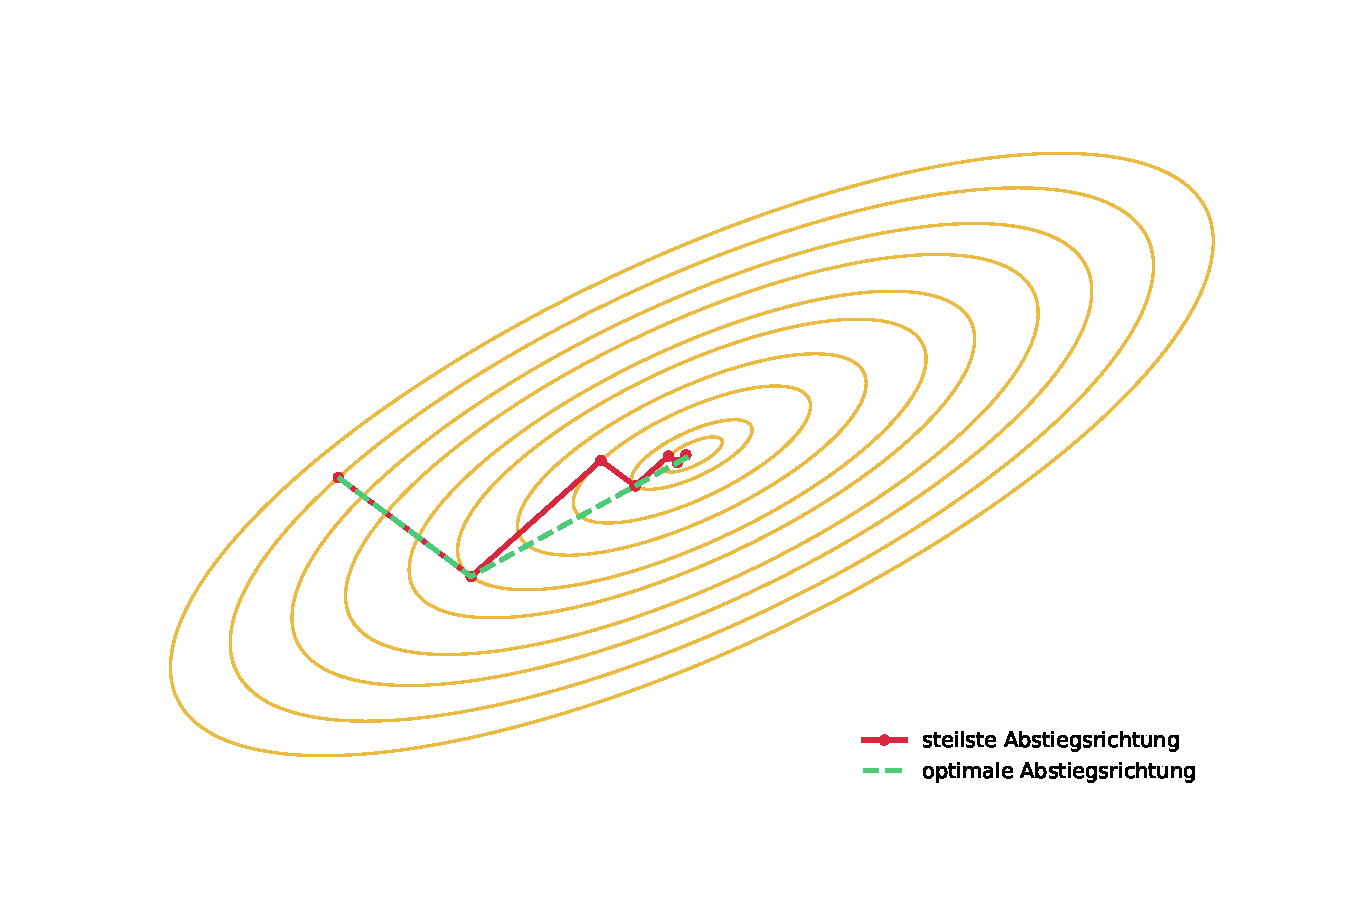
\includegraphics[width=0.9\linewidth,trim=50 40 50 50,clip]{figures/zickZackCourse.pdf}
\end{center}

\subsubsection{Das Verfahren der konjugierten Gradienten}
Die obige Idee kann zur effizienten Lösung linearer Gleichungssysteme genutzt werden.
Gegeben sei das LGS $Ax=b$ mit $A\in\K^{n\times n}$ hermetisch
($a_{ij}=\overline{a_{ji}}$). Das impliziert insbesondere, dass die Hauptdiagonale reell ist, und dass $x^HAy = y^HAx$ 
für $x,y\in\K^n$ gilt.

Zur Lösung wird dieses Mal die Minimierung folgendes quadratischen Funktionals betrachtet
%
\begin{align*}
  \phi(x)
  = \tfrac{1}{2}x^H A x - x^H b
  \tag{1}\label{eq:CGVeq1}
\end{align*}
%
Denn sollte eine Lösung $\hat{x}=A^{-1}b$ des LGS $Ax=b$ existieren, so gilt für alle $x\in\K^{n}$:
%
\begin{align*}
  &\phi(x)-\phi(\hat{x}) \\
  =& \tfrac{1}{2}x^H A x - x^H b - (\tfrac{1}{2}\hat{x}^H A \hat{x} - \hat{x}^H b) \\
  =&  \highlight{mypurple}{\tfrac{1}{2}x^H A x} 
      - x^H b 
      - (\highlight{myred}{\tfrac{1}{2}\hat{x}^H A \hat{x}} 
      - \hat{x}^H b) 
      + \overbrace{
        \tfrac{1}{2}(x-\hat{x})^H A (x-\hat{x}) 
        \highlight{mypurple}{- \tfrac{1}{2} x^H A x}
        \highlight{myyellow}{+ \tfrac{1}{2}x^H A \hat{x}}
        \highlight{myyellow}{+ \tfrac{1}{2} \hat{x}^H A x}
        \highlight{myred}{- \tfrac{1}{2}\hat{x}^H A \hat{x}}
  }^{=0} \\
  =& -x^H b + \hat{x}^H b + \tfrac{1}{2}(x-\hat{x})^H A (x-\hat{x}) 
  \highlight{myred}{- \hat{x}^H A \hat{x}} + \highlight{myyellow}{x^H A \hat{x}} \\
  =& -x^H b + \hat{x}^H b + \tfrac{1}{2}(x-\hat{x})^H A (x-\hat{x})  - \hat{x}^H b + x^H b \\
  =& \tfrac{1}{2} (x-\hat{x})^H A(x-\hat{x}) \\
  \geq& 0
\end{align*}
%
Die Funktion hat demnach ein eindeutiges Minimum bei $\hat{x}$.

\begin{colbox}{Definition}
  Ist $A\in\K^{n\times n}$ hermetisch und pos. definitiv, dann wird durch $\vertn{2}{x}_A=\sqrt{x^HAx}, 
  x\in\K^{n}$ eine Norm in $\K^n$ definiert, die sogenannte Energienorm. 
  Zur Energienorm gehört ein inneres Produkt $\langle x,y\rangle_A=x^HAy, x,y\in\K^n$.
  Es ergibt sich die Abweichung des Funktionals von seinem Minimum als:
  %
  \begin{align*}
    \phi(x)-\phi(\hat{x}) 
    = \tfrac{1}{2}\vertn{2}{x-\hat{x}}^2_A
    \tag{2}\label{eq:CGVeq2}
  \end{align*}
  %
\end{colbox}

\textbf{geometrische Interpretation:} Der Graph von $\phi$ bezüglich der Energienorm ist ein kreisförmiger Paraboloid, 
welcher über dem Mittelpunkt $\hat{x}$ liegt. 

\textbf{Idee:} Konstruktion eines Verfahrens, welches die Lösung $\hat{x}$ von $Ax=b$ iterativ approximiert, 
indem das Funktional $\phi$ sukzessiv minimiert wird: 

Zur aktuellen Iteration $x^{(k)}$ wird die Suchrichtung $d^{(k)}\neq 0$ bestimmt, und die neue Iterierte 
$x^{(k+1)}$ über den Ansatz
% 
\begin{align*}
  x^{(k+1)} 
  = x^{(k)} + \alpha\cdot d^{(k)} 
  \tag{3}\label{eq:CGVeq3}
\end{align*}
%
bestimmt (gleiche Ansatz wie zuvor). Es gilt dann
%
\begin{align*}
  \phi(x^{(k)}+\alpha d^{(k)}) 
  = \phi(x^{(k)}) + \alpha d^{(k)H}A x^{(k)} + \tfrac{1}{2}\alpha^2 {d^{(k)H}}Ad^{(k)}-\alpha{d^{(k)H}}\cdot b 
  \tag{4}\label{eq:CGVeq4}
\end{align*}
%
Durch Differentiation nach $\alpha$ und Null setzen der Ableitung ergibt sich unsere Schrittweite $\alpha^{(k)}$:
%
\begin{align*}
  \alpha^{(k)} 
  = \dfrac{{r^{(k)H}} d^{(k)}}{{d^{(k)H}} A d^{(k)}},
  \qquad \text{mit } 
  r^{(k)}
  = b-Ax^{(k)} 
  \tag{5}\label{eq:CGVeq5}
\end{align*}
zusätzlich erhalten wir die Suchrichtung $d^{(k)}$ indem wir die Richtungsableitung von $\phi$ betrachten, dabei gilt:
%
\begin{align*}
  \dfrac{\partial}{\partial d^{(k)}} \phi(x^{(k)}) 
  &= \lim_{\alpha\to 0} \dfrac{\phi(x^{(k)}+\alpha d^{(k)}) - \phi(x^{(k)})}{\alpha} \\
  &\stackrel{(4)}{=} \lim_{\alpha\to 0} 
  \dfrac{\alpha d^{(k)H}A x^{(k)} + \tfrac{1}{2}\alpha^2 {d^{(k)H}}Ad^{(k)}-\alpha{d^{(k)H}}\cdot b}{\alpha} \\
  &= d^{(k)H}(Ax^{(k)}-b) + \lim_{\alpha\to 0} \tfrac{1}{2}\alpha {d^{(k)H}}Ad^{(k)} \\
  &= -d^{(k)H}r^{(k)}
\end{align*}
%
Ziel ist es nun die Idee des Verfahren des steilsten Abstiegs zu verbessern, indem wir nicht nur in Richtung 
$r^{(k)}$ wandern (was zwar der größtmögliche Abstieg wäre, aber unvorteilhaftes \glqq{}Zick-Zack-Verhalten\grqq{} 
mit sich bringt), sondern stattdessen 
%
\begin{align*}
  d^{(k)} = r^{(k)} + \beta^{(k-1)} d^{(k-1)}
  \tag{6}\label{eq:CGVeq6}
\end{align*}
%
Dabei sollte $\beta^{(k-1)}$ gerade so gewählt sein, dass 
$d^{(k)}$ und $d^{(k-1)}$ konjugiert bezüglich $A$ sind, d.h. $\langle d^{(k-1)}, d^{(k)} \rangle = 0$. Aus dieser 
Bedingung ergibt sich dann 
%
\begin{align*}
  \beta^{(k-1)} &= -\dfrac{r^{(k)H}Ad^{(k-1)}}{d^{(k-1)H}Ad^{(k-1)}} 
  \tag{7}\label{eq:CGVeq7}
\end{align*}

Die Gleichungen (\ref{eq:CGVeq5}) und (\ref{eq:CGVeq7}) sind wohldefiniert, wenn ${d^{(k)H}}Ad^{(k)}\neq 0$, 
aufgrund der positiv Definitheit von $A$ ist dies genau dann der Fall wenn $d^{(k)}\neq 0$. 

Nach (\ref{eq:CGVeq6}) ist $d^{(k)} = 0$ jedoch nur dann möglich, wenn $r^{(k)}$ und $d^{(k-1)}$ linear abhängig sind, 
doch nach Konstruktion verläuft die Suchrichtung $d^{(k-1)}$ tangential zur Niveaufläche von $\phi$, 
also orthogonal zum Gradienten $r^{(k)}$.

Somit folgt $d^{(k)} = 0$ nur wenn $r^{(k)}=0$, was $x^{(k)}=\hat{x}$ implizieren würde. 

\subsubsection{Eigenschaften des CG-Verfahrens}
Wegen der Orthogonalitätsbedingung $\langle d^{(k+1)},d^{(k)}\rangle_A=0$ nennt man die 
Suchrichtungen zueinander $A$-konjugiert und das Verfahren, Verfahren der konjugierten Gradienten (CG-Verfahren). 
Zusätzlich zur Konjugiertheit von sukzessiven Suchrichtungen ergeben sich folgende weitere Eigenschaften:

\begin{colbox}{Lemma}\label{lem:CGVprop}
  Sei $x^{(0)}$ ein beliebiger Startvektor und $d^{(0)}=r^{(0)}=b-Ax^{(0)}$. \\
  Wenn $x^{(k)}\neq \hat{x}$ für $k=0,1,\dots, m$, mit $A\hat{x}=b$, so gilt:
  \begin{enumerate}
    \item[a)] ${r^{(m)H}}d^{(j)}=0$ für $0\leq j < m$
    \item[b)] ${r^{(m)H}}r^{(j)}=0$ für $0\leq j < m$ 
    \item[b)] $\langle d^{(m)}, d^{(j)}\rangle_A=0$ für $0\leq j < m$ \qquad (10)\label{eq:CGVeq10}
  \end{enumerate}
\end{colbox}

\textit{Beweis.} \\
Für $k\geq 0$ gilt mit (\ref{eq:CGVeq3}), dass $Ax^{(k+1)} = Ax^{(k)} + \alpha^{(k)} Ad^{(k)}$ und somit 
%
\begin{align*}
  r^{(k+1)} 
  &= b - Ax^{(k+1)} \\
  &= b - Ax^{(k)} - \alpha^{(k)} Ad^{(k)}\\
  &= r^{(k)}-\alpha^{(k)}Ad^{(k)}
  \tag{8}\label{eq:CGVeq8}
\end{align*}
%
die nach (\ref{eq:CGVeq5}) definierte optimale Wahl für $\alpha$ bewirkt dann, dass
%
\begin{align*}
  {r^{(k+1)H}}d^{(k)} &= (r^{(k)}-\alpha^{(k)}Ad^{(k)})^H d^{(k)} \\
  &= {r^{(k)H}} d^{(k)} - \alpha^{(k)}{d^{(k)H}}Ad^{(k)} \\
  &= {r^{(k)H}} d^{(k)} - \dfrac{{r^{(k)H}} d^{(k)}}{d^{(k)H}Ad^{(k)}} d^{(k)H}Ad^{(k)} \\
  &\stackrel{(5)}{=} 0 
  \tag{9}\label{eq:CGVeq9}
\end{align*}
%
Weiter gilt nach Induktion über $m$: 

\underline{Induktionsanfang:} $m=1$. \\
Durch die Wahl $k=0$ in (\ref{eq:CGVeq9}) erhalten wir die Behauptung (a) 
und nach Setzung $d^{(0)}=r{(0)}$ auch die Behauptung (b). (c) folgt im Fall $m=1$ direkt aus der 
Orthogonalitätsbedingung. 

\underline{Induktionsschritt:} $m\rightarrow m+1$. \\
Wir nehmen an, dass die Aussagen (a), (b) und (c) 
für $m\leq\overline{m}$ richtig sind und zeigen damit die Gültigkeit für $m=\overline{m}+1$. \\
Zunächst folgt aus (\ref{eq:CGVeq9}) mit $k=\overline{m}$, dass ${r^{(\overline{m}+1)H}}d^{(\overline{m})} = 0$, 
sowie aus der Darstellungen $r^{(m+1)}$ von (\ref{eq:CGVeq8}) mit der Induktionsannahme (a und c):
%
\begin{align*}
  {r^{(\overline{m}+1)H}}d^{(j)} 
  = {r^{(\overline{m})H}}d^{(j)} - \alpha^{(\overline{m})}\langle d^{(\overline{m})}, d^{(j)} \rangle_A 
  = 0 
  \text{ für } 0\leq j < \overline{m}
\end{align*}
%
Damit gilt (a) auch für $m=\overline{m}+1$. 

Weiter ergibt (\ref{eq:CGVeq6}) umgestellt $r^{(j)} = d^{(j)} - \beta^{(j-1)}d^{(j-1)}$ und mit $r^{(0)}=d^{(0)}$ folgt 
daher (b) rekursiv aus (a):
%
\begin{align*}
  {r^{(\overline{m}+1)H}}r^{(j)} 
  = {r^{(\overline{m}+1)H}}d^{(j)} - \beta^{(j-1)}\cdot {r^{(\overline{m}+1)H}}d^{(j-1)} 
  = 0 - \beta^{(j-1)}\cdot 0 
  = 0
\end{align*}
%
Damit (c) gilt muss noch $\alpha^{(j)}\neq 0$ für $j<\overline{m}$ sein (der Fall $j=\overline{m}$ ergibt sich direkt aus 
der Orthogonalitätsbedingung), denn dann ergibt (\ref{eq:CGVeq8}):
%
\begin{align*}
  Ad^{(j)} = \dfrac{1}{\alpha^{(j)}} \left(r^{(j+1)}- r^{(j)}\right)
\end{align*}
%
und somit folgt durch (\ref{eq:CGVeq6}):
%
\begin{align*}
  \langle d^{(\overline{m}+1)}, d^{(j)}\rangle_A 
  &= \langle r^{(\overline{m}+1)}, d^{(j)}\rangle_A 
  + \beta^{(\overline{m})}\underbrace{\langle d^{(\overline{m})}, d^{(j)}\rangle_A}_{=0}\\
  &= {r^{(\overline{m}+1)H}}Ad^{(j)} \\
  &= r^{(\overline{m}+1)H}\cdot\dfrac{1}{\alpha^{(j)}} \left(r^{(j+1)}- r^{(j)}\right) \\
  &= \dfrac{1}{\alpha^{(j)}} 
  \Big(\underbrace{r^{(\overline{m}+1)H}r^{(j+1)}}_{=0} - \underbrace{r^{(\overline{m}+1)H}r^{(j)}}_{=0}\Big) \\
  &= 0 
\end{align*}
%
Angenommen $\alpha^{(j)} = 0$, dann folgt aus der Definition von $\alpha^{(j)}$ (\ref{eq:CGVeq5}), 
dass auch ${r^{(j)H}}d^{(j)}=0$ und mit (\ref{eq:CGVeq6}) 
%
\begin{align*}
  0 = {r^{(j)H}}d^{(j)}
  = {r^{(j)H}}\left(r^{(j)}+\beta^{j-1}d^{(j-1)}\right) 
  = {r^{(j)H}}r^{(j)}+\beta^{(j-1)}\underbrace{{r^{(j)H}}d^{(j-1)}}_{=0} 
  = \vertn{2}{r^{(j)}}_2^2
\end{align*}
Das impliziert $r^{(j)} = 0$, doch dann wäre aber $x^{(j)}=\hat{x}$ (Widerspruch). \qed 

Das Lemma sagt insbesondere aus, dass alle Suchrichtungen paarweise $A$-konjugiert. Außerdem bilden 
die Residuen ein Orthogonalsystem und sind damit linear unabhängig.
Es muss sich daher nach spätestens $n$ Schritten $r^{(n)}=0$, also $x^{(n)}=\hat{x}$ ergeben.

\begin{colbox}{Korollar}\label{cor:CGVconvn}
  Für $A\in\K^{n\times n}$ hermetisch und positiv definit findet das CG-Verfahren nach 
  höchstens $n$ Schritten die exakte Lösung $x^{(n)}=\hat{x}$.
\end{colbox}

In der Praxis ist dieses Korollar nicht relevant, da häufig wesentlich weniger Schritte benötigt werden oder die 
Orthogonalitätsbedingung aufgrund von Rundungsfehlern verloren gehen.

Eine alternative Interpretation als iteratives Verfahren (neben der geometrischen Idee) bietet die Theorie über 
Krylov-Räume:

\begin{colbox}{Definition}
  Sei $A\in\K^{n\times n}$ und $y\in\K^n$. Dann heißt der Unterraum 
  \begin{align*}
    \mathcal{K}_k(A,y) := \Span\{y,Ay,\dots,A^{k-1}y\}\leq \K^n
  \end{align*} 
  Krylov-Raum der Dimension $k$ von $A$ bezüglich $y$.
\end{colbox}

\begin{colbox}{Satz}\label{satz:CGVkrylov}
  Sei $A\in\K^{n\times n}$ hermetisch und positiv definit, $d^{(0)}=r^{(0)}$, und $x^{(k)}\neq \hat{x}$ 
  die $k$-te Iterierte des CG-Verfahrens. 
  Dann gilt 
  %
  \begin{align*}
    x^{(k)}\in x^{(0)} + \mathcal{K}_k(A,r^{(0)})
  \end{align*}
  %
  und $x^{(k)}$ ist 
  in diesem affinen Raum die eindeutige Minimalstelle der Zielfunktion $\phi$. (Optimalitätseigenschaft)
\end{colbox}

\textit{Beweis.} 
\begin{enumerate}
  \item[a)] Wir beginnen damit induktiv zu zeigen, dass 
  %
  \begin{align*}
    d^{(j)}\in\Span\{r^{(0)}, \dots, r^{(j)}\} \qquad \text{für } j=0,\dots,k+1 
    \tag{11}\label{eq:CGVeq11}
  \end{align*}
  %
  \underline{Induktionsanfang:} $j=0$. \\
  Wegen $d^{(0)}=r^{(0)}$ offensichtlich erfüllt.  \\
  \underline{Induktionsschritt:} $j\rightarrow j+1$. Folgt direkt aus der Rekursionsvorschrift für $d$ 
  (\ref{eq:CGVeq6}):
  %
  \begin{align*}
    d^{(j+1)} 
    = r^{(j+1)} + \beta^{(j)}\cdot d^{(j)} 
    = r^{(j+1)} + \beta^{(j)}\sum_{i=0}^{j}\delta_i r^{(i)}
    \in \Span\{r^{(0)}, \dots, r^{(j+1)}\}
  \end{align*}

  Es folgt damit $\Span\{d^{(0)}, \dots, r^{(k-1)}\}\subset\Span\{r^{(0)}, \dots, r^{(k-1)}\}$
  Zusammen mit dem Lemma \ref{lem:CGVprop} folgt dass beide Systeme jeweils linear unabhängig sind, also jeweils 
  Dimension $k-1$ haben, wodurch Gleichheit gilt.
  %
  \begin{align*}
    \Span\{d^{(0)}, \dots, r^{(k-1)}\} = \Span\{r^{(0)}, \dots, r^{(k-1)}\}
  \end{align*}
  %
  Aus der Rekursionsformel von $x$ (\ref{eq:CGVeq3}) ergibt sich der explizit Ausdruck:
  %
  \begin{align*}
    x^{(k)} 
    = x^{(0)} + \sum_{j=0}^{k-1} \alpha^{(j)}\cdot d^{(j)} 
    \in x^{(0)} + \Span\{r^{(0)}, \dots, r^{(k-1)}\},
    \quad\text{für } j=0,\dots,k-1
  \end{align*}
  %
  Im nächsten Schritt wird induktiv gezeigt, dass $r^{(j)}\in \mathcal{K}_j(A,r^{(0)})$: 

  \underline{Induktionsanfang:} $j=0$. \\
  Offensichtlich gilt $r^{(0)}\in\text{span}\{r^{(0)}\}$.
  \underline{Induktionsschritt: } $j-1\rightarrow j$.\\
  Aus Teil (a) und der Induktionsannahme folgt 
  %
  \begin{align*}
  & d^{(j-1)}\in\text{span}\{r^{(0)}, \dots, r^{(j-1)}\}
  \subset \text{span}\{r^{(0)}, \dots, A^{j-1}r^{(0)}\} \\
  \xRightarrow{(8)} \quad
  & r^{(j)} = r^{(j-1)}-\alpha^{(j-1)}Ad^{(j-1)}
  \in \text{span}\{r^{(0)}, \dots, A^{j}r^{(0)}\}
  \end{align*}
  %
  Damit folgt $\Span\{r^{(0)},\dots,r^{(k-1)}\}\subset \mathcal{K}_j(A,r^{(0)})$. 
  Die Menge $\{r^{(j)}\}_{j=0}^{k-1}$ ist linear unabhängig und daher hat der linke Unterraum die Dimension $k$, 
  es folgt Gleichheit 
  %
  \begin{align*}
      \Span\{d^{(0)}, \dots, r^{(k-1)}\} = \Span\{r^{(0)}, \dots, r^{(k-1)}\} = \mathcal{K}_j(A,r^{(0)})
  \end{align*}
  %
  und damit auch $x^{(k)}\in x^{(0)} + \mathcal{K}_k(A,r^{(0)})$.

  \item[c)] 
  Aus Korollar \ref{cor:CGVconvn} folgt die Existenz eines Iterationsindex $m\leq n$ mit 
  %
  \begin{align*}
    \hat{x} 
    = x^{(0)} + \sum_{j=0}^{m-1} \alpha^{(j)}\cdot d^{(j)}
  \end{align*}
  %
  Für ein $0\leq k\leq m$ gilt dann:
  %
  \begin{align*}
    \hat{x}
    = x^{(0)} + \sum_{j=0}^{k-1} \alpha^{(j)}\cdot d^{(j)} + \sum_{j=k}^{m-1} \alpha^{(j)}\cdot d^{(j)} 
    = x^{(k)} + \sum_{j=k}^{m-1} \alpha^{(j)}\cdot d^{(j)}
  \end{align*}
  %
  Und für ein beliebiges $x\in x^{(0)} + \mathcal{K}_k(A,r^{(0)}) = x^{(0)} + \Span\{d^{(0)},\dots,d^{(k-1)}\}$ 
  demnach
  % 
  \begin{align*}
    \hat{x}-x 
    & = \hat{x}-x^{(k)}+x^{(k)}-x \\
    & = x^{(0)} + \sum_{j=1}^{m-1}\alpha^{(j)}\cdot d^{(j)} 
    - \sum_{j=0}^{k-1} \alpha^{(j)}\cdot d^{(j)} 
    + \sum_{j=0}^{k-1} \alpha^{(j)}\cdot d^{(j)} 
    - x^{(0)} - \sum_{j=0}^{k-1}\delta_j\cdot d^{(j)}\\
    & = \sum_{j=k}^{m-1}\alpha^{(j)}\cdot d^{(j)} + \sum_{j=0}^{k-1}(-\alpha^{(j)}-\delta_j)\cdot d^{(j)} \\
    & = \hat{x} - x^{(k)} + \sum_{j=0}^{k-1}(-\alpha^{(j)}-\delta_j)\cdot d^{(j)} \\
  \end{align*}
  %
  für $\delta_j\in\K$. Da die Suchrichtungen nach Lemma \ref{lem:CGVprop} $A$-konjugiert sind folgt:
  %
  \begin{align*}
    \phi(x) - \phi(\hat{x})
    &= \tfrac{1}{2}\vertn{2}{\hat{x}-x}_A^2 \\
    &= \dfrac{1}{2}\vertn{2}{\sum_{j=k}^{m-1}\alpha^{(j)}\cdot d^{(j)} 
    + \sum_{j=0}^{k-1}(-\alpha^{(j)}-\delta_j)\cdot d^{(j)}}_A^2 \\
    &= \dfrac{1}{2}\vertn{2}{\sum_{j=k}^{m-1}\alpha^{(j)}\cdot d^{(j)}}_A^2 
    + \dfrac{1}{2}\vertn{2}{\sum_{j=0}^{k-1}(-\alpha^{(j)}-\delta_j)\cdot d^{(j)}}_A^2 \\
    &= \tfrac{1}{2}\vertn{2}{\hat{x}-x^{(k)}}_A^2 
    + \dfrac{1}{2}\vertn{2}{\sum_{j=0}^{k-1}(-\alpha^{(j)}-\delta_j)\cdot d^{(j)}}_A^2 \\
    &= \phi(\hat{x}) - \phi(x^{(k)}) + \dfrac{1}{2}\vertn{2}{\sum_{j=0}^{k-1}(-\alpha^{(j)}-\delta_j)\cdot d^{(j)}}_A^2 \\
    &\geq \phi(\hat{x}) - \phi(x^{(k)})
  \end{align*}
  %
  Insbesondere gilt Gleichheit bei $x=x^{(k)}$.
  \qed
\end{enumerate}

\subsubsection{Praktische Aspekte der Implementierung}
\begin{colbox}{Bemerkung}
  Für eine Implementierung des CG-Verfahren sollte man nicht die Gleichungen (5) und (7) für $\alpha^{(k)}$ 
  und $\beta^{(k)}$ verwenden, sondern lieber folgende Darstellungen, welche numerisch stabiler sind:
  %
  \begin{align*}
    \alpha^{(k)} &= \dfrac{\vertn{2}{r^{(k)}}_2^2}{{d^{(k)H}}Ad^{(k)}} \tag{5'}\label{eq:CGVeq5*} \\
    \beta^{(k)} &= \dfrac{\vertn{2}{r^{(k+1)}}_2^2}{\vertn{2}{r^{(k)}}_2^2} \tag{7'}\label{eq:CGVeq7*}
  \end{align*}
\end{colbox}
Die Gleichung (\ref{eq:CGVeq5*}) folgt aus (\ref{eq:CGVeq3}) und Lemma \ref{lem:CGVprop} (a), nach welchen
%
\begin{align*}
  {r^{(k)H}}d^{(k)} 
  = {r^{(k)H}}r^{(k)} + \beta^{(k)}\cdot \underbrace{{r^{(k)H}}d^{(k-1)}}{=0}
  = \vertn{2}{r^{(k)}}_2^2
\end{align*}
%
Die Gleichung (\ref{eq:CGVeq7*}) folgt dann aus aus (\ref{eq:CGVeq8}), (\ref{eq:CGVeq5*}) 
und dem Lemma \ref{lem:CGVprop} (b):
%
\begin{align*}
  {r^{(k+1)H}}Ad^{(k)} 
  = \dfrac{1}{\alpha^{(k)}}\left({r^{(k+1)H}}r^{(k)} - {r^{(k+1)H}}r^{(k+1)}\right) 
  =\dfrac{-\vertn{2}{r^{(k+1)}}_2^2}{\alpha^{(k)}} 
  = -\dfrac{\vertn{2}{r^{(k+1)}}_2^2}{\vertn{2}{r^{(k)}}_2^2}{d^{(k)H}}Ad^{(k)}
\end{align*} 

Es ergibt sich damit folgender Algorithmus:

\algorithmbox{CG-Verfahren}{
\begin{algorithm}[H]
  \SetAlgoNoLine
  \InitTe{$A\in \K^{n\times n}$ sei hermetisch und positiv definit.}
  \ErgTe{
    $x^{(k)}$ als Approximation für $A^{-1}b$, 
    \newline $r^{(k)}=b-Ax^{(k)}$ als zugehöriges Residuum.
  } 
  \SetAlgoLined
  Wähle $x^{(0)}\in\K^{n}$ beliebig \\
  $r^{(0)} \leftarrow b-Ax^{(0)}$ \\
  $d^{(0)} \leftarrow r^{(0)}$ \\
  \ForTe{$k=0,1,\dots,$}{
    $\alpha^{(k)} \leftarrow \dfrac{\vertn{2}{r^{(k)}}_2^2}{{d^{(k)H}}Ad^{(k)}}$ \\
    $x^{(k+1)} \leftarrow x^{(k)} + \alpha^{(k)}d^{(k)}$ \\
    $r^{(k+1)} \leftarrow r^{(k)} - \alpha^{(k)}Ad^{(k)}$ \\
    $\beta^{(k)} \leftarrow \dfrac{\vertn{2}{r^{(k+1)}}_2^2}{\vertn{2}{r^{(k)}}_2^2}$ \\
    $d^{(k+1)} \leftarrow r^{(k+1)} + \beta^{(k)}d^{(k)}$
  }
  \SetAlgoNoLine
  \UntilStopTe{}{}
\end{algorithm}
}

Der Aufwand des CG-Verfahrens ergibt sich aus einer Matrix-Vektor Multiplikation in jedem Iterationsschritt 
und ist damit vergleichbar mit dem Gesamt -und Einzelschritt.

\begin{colbox}{Bemerkung}
  Das CG-Verfahren ist typischerweise wesentlich schneller als das Gesamt -bzw. Einzelschrittverfahren, 
  \textbf{aber} verlangt, dass die vorausgesetzte Matrix hermetisch ist. \\
  Ein schnelles und einfaches Verfahren für allgemeine Matrizen ist derzeit nicht bekannt, ein komplizierteres 
  Verfahren mit ähnlicher Konvergenzgeschwindigkeit ist das GMRES-Verfahren 
  (Vgl. Hanku-Bourgeois, Kapitel 3, Abschnitt 16). 
\end{colbox}

\subsection{Präkonditionierung des CG-Verfahren}

\begin{colbox}{Definition}
  $\kappa_M(A) = \cond_M(A) = \vertn{2}{A^{-1}}_M\cdot \vertn{2}{A}_M$ wird als Kondition der Matrix $A$ bezüglich 
  der Norm $\vertn{2}{\cdot}_M$ bezeichnet. 
  Sie beschreibt die schlimmstmögliche Fortpflanzung des Eingangsfehlers beim Lösen eines LGS.
\end{colbox}

Gegeben sei $Az=b$ mit der Lösung $z=A^{-1}b$. Der Einfluss vom Eingangsfehlers sei $\Delta b$:
%
\begin{align*}
  z + \Delta z 
  = A^{-1}(b+\Delta b) 
  = A^{-1}b + A^{-1}\Delta b
\end{align*}
Die berechnete Lösung erhält dabei den Fortpflanzungsfehler $\Delta z = A^{-1}\Delta b$. 

Sei $\vertn{2}{\cdot}$ die zu $\vertn{2}{\cdot}_M$ verträgliche Matrixnorm 
(d.h. $\vertn{2}{Ax}\leq \vertn{2}{A}_M\cdot\vertn{2}{x}$), 
so ergibt sich als relativer Fehler:
%
\begin{align*}
  \dfrac{\vertn{2}{\Delta z}}{\vertn{2}{z}} 
  &= \dfrac{\vertn{2}{\Delta z}}{\vertn{2}{b}} \cdot\dfrac{\vertn{2}{b}}{\vertn{2}{z}} \\
  &= \dfrac{\vertn{2}{A^{-1}\Delta b}}{\vertn{2}{b}} \cdot\dfrac{\vertn{2}{Az}}{\vertn{2}{z}} \\
  &\leq \vertn{2}{A^{-1}}_M \cdot \vertn{2}{A}_M \cdot \dfrac{\vertn{2}{\Delta b}}{\vertn{2}{b}} 
  \cdot \dfrac{\vertn{2}{z}}{\vertn{2}{z}} \\
  &= \cond_M{A}\cdot\dfrac{\vertn{2}{\Delta b}}{\vertn{2}{b}} \\
\end{align*}
%
Typischerweise ist die Konvergenz eines numerischen Verfahrens umso langsamer, je schlechter die Matrix $A$ 
konditioniert ist, d.h. je größer die Konditionszahl $A$ ist.

\subsubsection{Präkonditionierung mittels Cholesky}
\textbf{Idee:} 
Gleichungssystem $Ax=b$ in ein äquivalentes LGS umwandeln, sodass die Kondition sich verbessert: 
  \begin{align*}
    M^{-1}Ax = M^{-1}b  \tag{{\scriptsize$\triangle$}} \label{eq:präForm}
  \end{align*}
wobei $M$ hermetisch und positiv definit ist. 

\textbf{Problem:} 
Die Matrix $M^{-1}A$ muss nicht notwendig hermetisch sein, daher nutzen wir die 
Cholesky-Zerlegung $M=LL^H$
und erhalten\footnote{$L^{-H} = (L^H)^{-1} = (L^{-1})^H$}: 
%
\begin{align*}
  L^{-H}L^{-1}Ax = L^{-H}L^{-1}b \implies L^{-1}AL^{-*}z = L^{-1}b \quad \text{mit } x = L^{-*}z
\end{align*}
%
Hierbei ist die Koeffizientenmatrix $L^{-1}AL^{-H}$ sicher hermetisch und positiv definit, 
denn $(L^{-1}AL^{-H})^H = (L^{-H})^HA^H(L^{-1})^H = L^{-1}AL^{-H}$ und für beliebiges 
$z\in\K^n$ und $x=L^{-H}z$ gilt: 
%
\begin{align*}
  z^HL^{-1}AL^{-H}z 
  = x^HL^{-H}z 
  = x^HAx \geq 0
\end{align*}
%
Wir können also CG-Verfahren zum Lösen von $L^{-1}AL^{-*}z = L^{-1}b$ nutzen und aus dieser Lösung 
dann $x$ bestimmen. In der Praxis werden wir stattdessen durch geschickte Modifikation des klassischen 
CG-Verfahren direkt $x$ berechnen.

\textbf{Ziel:} Die Konditionszahl von $L^{-1}AL^{-*}$ soll kleiner werden als die Konditionszahl von $A$, dies 
liefert schnellere Konvergenz der Iterierten $z^{(k)}$ und der Lösung $x^{(k)}=L^{-*}z$ 

\begin{colbox}{Bemerkung}
  Die Faktorisierung $M=LL^H$ muss nicht explizit berechnet werden, 
  da die Variable $z$ wieder durch $x$ substituiert werden kann.

  Für die Berechnung der Koeffizienten $\beta^{(k)}$ und die dafür benötigte Norm 
  $\vertn{2}{L^{-1}b-L^{-1}AL^{-H}z^{(k)}}_2^2$ wird neben $r^{(k)} = b-A^{(k)}$ noch ein Hilfsvektor 
  \begin{align*}
    s^{(k)} = M^{-1}r^{(k)} = M^{-1}b - M^{-1}Ax^{(k)}
  \end{align*}
  benötigt ($s^{(k)}$ beschreibt das Residuum von (\ref{eq:präForm})).
  
  Für die Norm gilt 
  %
  \begin{align*}
    \vertn{2}{L^{-1}b-L^{-1}AL^{-H}z^{(k)}}_2^2 
    = \Big\|{L^{-1}\underbrace{(b-Ax^{(k)})}_{=r^{(k)}}}\Big\|_2^2
    = ({r^{(k)H}}\underbrace{L^{-H})(L^{-1}r^{(k)}}_{=s^{(k)}}) 
    = {r^{(k)H}}s^{(k)}
  \end{align*}
  %
\end{colbox}

\subsubsection{Algorithmus: PCG-Verfahren}
\algorithmbox{Präkonditioniertes CG-Verfahren (PCGV)}{
\begin{algorithm}[H]
  \SetAlgoNoLine
  \InitTe{$A,M\in \K^{n\times n}$ seien hermetisch und positiv definit.}
  \ErgTe{$x^{(k)}$ als Approximation für $A^{-1}b$, 
  \newline $r^{(k)}=b-Ax^{(k)}$ Residuum im Schritt $k$,
  \newline $s^{(k)}$ das Residuum von ({\scriptsize$\triangle$}).} 
  \SetAlgoLined
  Wähle $x^{(0)}\in\K^{n}$ beliebig \\
  $r^{(0)} \leftarrow b-Ax^{(0)}$ \\
  Löse $Ms^{(0)} = r^{(0)}$ \\
  $d^{(0)} \leftarrow s^{(0)}$ \\
  \ForTe{$k=0,1,\dots,$}{
    $\alpha^{(k)} \leftarrow \dfrac{{r^{(k)H}}s^{(k)}}{{d^{(k)H}}Ad^{(k)}}$ \\
    $x^{(k+1)} \leftarrow x^{(k)} + \alpha^{(k)}d^{(k)}$ \\
    $r^{(k+1)} \leftarrow r^{(k)} - \alpha^{(k)}Ad^{(k)}$ \\
    Löse $Ms^{(k+1)} = r^{(k+1)}$ \\
    $\beta^{(k)} \leftarrow \dfrac{{r^{(k+1)H}}s^{(k+1)}}{{r^{(k)H}}s^{(k)}}$ \\
    $d^{(k+1)} \leftarrow s^{(k+1)} + \beta^{(k)}d^{(k)}$
  }
  \SetAlgoNoLine
  \UntilStopTe{}{}
\end{algorithm}
}

Der Aufwand im Vergleich zum CGV erhöht sich beim PCGV um das Lösen eines LGS $Ms=r$. Die erhoffte schnellere
Konvergenz des Iterationsverfahren macht sich also nur bezahlt, wenn das LGS $Ms=r$ entsprechend billig gelöst
werden kann. 

Da $A$ bei Anwendung des CGV typischerweise dünn besetzt ist, dominieren die Kosten für die Lösung des LGS $Ms=r$ 
bei dem Gesamtkosten des PCGV.

\begin{colbox}{Satz}
  Die $k$-te Iterierte $x^{(k)}$ vom Algorithmus des PCGV liegt in dem affin verschobene Krylov-Raum
  $x^{(0)} + \mathcal{K}_k(M^{-1}A, M^{-1}r^{(0)})$ und ist in dieser Menge die eindeutig bestimmte Minimalstelle
  des Funktionals $\phi(x) = \tfrac{1}{2}x^HAx-x^Hb$.
\end{colbox}

\textit{Beweis.} %(Vgl. Beweis zu Satz \ref{satz:CGVkrylov})

Nach Satz \ref{satz:CGVkrylov} liegt die entsprechende Iterierte $z^{(k)}=L^Hx^{(k)}$ in dem affin 
verschobenen Krylov-Raum $z^{(0)} + \mathcal{K}_k(L^{-1}AL^{-H}, L^{-1}b-L^{-1}AL^{-1}z^{(0)})$ 
mit $z^{(0)} = L^Hx^{(0)}$ und minimiert in dieser Menge das Fehlerfunktional 
$\psi(z) = \tfrac{1}{2}L^{-1}AL^{-H}z-z^HL^{-1}b$. 

Durch die Transformation $x=L^{-H}z$ werden die Iterierten und die genannten Krylov-Räume aufeinander abgebildet
und es gilt $\psi(z) = \phi(x)$. \qed

\begin{colbox}{Bemerkung}
  Die Konstruktion geeigneter Präkonditionsmatrizen $M$ ist eine schwierige Sache.
\end{colbox}

\subsection{Anwendung und Konvergenzgeschwindigkeit des CG-Verfahren}
\subsubsection{Lösen von Randwertproblemen mittels CG-Verfahren}
Bevor wir zu einer Anwendung derartiger iterierten Verfahren starten, 
wiederholen wir kurz einen wichtigen Satz der Analysis:
\begin{colbox}{Satz}[Satz von Taylor]
  Sei $f:[a,b]\rightarrow \R$ eine $(n+1)$-mal stetig differenzierbare Funktion und $x,x_0\in[a,b]$. 
  Dann existiert ein $\xi$ zwischen $x$ und $x_0$, so dass
  \begin{align*}f(x) = \sum_{k=0}^{n}\dfrac{f^{(k)}(x_0)}{k!}(x-x_0)^k + 
  \underbrace{\dfrac{f^{(n+1)}(\xi)}{(n+1)!}\cdot(x-x_0)^{n+1}}_{R_n(x,x_0)}\end{align*}
\end{colbox}
\textit{Beweis.} Analysis II.

\begin{colboxBreakable}{Beispiel}\label{bsp:pdeBsp}
  Wir betrachten das Randwertproblem des Laplace Operators\footnote{
    Sei $f$ eine Funktion in kartesischen Koordinaten $(x,y)$, so ist der Laplace Operator definiert durch 
    %
    \begin{align*}
      \Delta f = \dfrac{\partial^2 f(x,y)}{\partial x^2} + \dfrac{\partial^2 f(x,y)}{\partial y^2}
    \end{align*}
    %
    }:
  %
  \begin{align*}
    -\dfrac{\partial^2 u(x,y)}{\partial x^2} 
    - \dfrac{\partial^2 u(x,y)}{\partial y^2} 
    = f(x,y) \quad 
    \text{ für } (x,y)\in Q
  \end{align*}
  %
  gemeinsam mit der Dirichlet-Randbedingung $u(x,y)=0$ für $(x,y)\in \partial Q$ auf dem Einheitsquadrat 
  $Q=(0,1)\times(0,1)\subset\R^2$. 

  Die Lösung $u=u(x,y)$ beschreibt z.B. die Auslenkung einer (idealisierten) Membran, die über dem Gebiet $Q$ 
  horizontal gespannt ist und mit einer Kraftdichte $f$ vertikal belastet wird. 

  Eine Lösung ist im Allgemeinen nicht analytisch angebbar, sodass man auf numerische Näherungslösungen 
  zurückgreifen muss.

  Betrachte $Q$ als Quadratgitter: 

  \begin{center}
    \begin{tikzpicture}[scale=0.5, thick, every node/.style={font=\large}]

  % Grid
  \draw[line width=1pt] (0,0) grid (6,6);

  % Center
  \def\x{3}
  \def\y{3}

  % Points
  \foreach \dx/\dy in {1/0, -1/0, 0/1, 0/-1}
  \fill[mydarkblue] (\x+\dx,\y+\dy) circle (4pt);
  \fill[mydarkred] (\x,\y) circle (4pt);

  % Labels
  \node (toplabel)   [mydarkblue] at (\x+5,\y+1.5) {$(x, y{+}h)$};
  \node (centerlabel)[mydarkred]  at (\x+4.6,\y+0.5)   {$(x, y)$};
  \node (rightlabel) [mydarkblue] at (\x+5,\y-0.5) {$(x{+}h, y)$};
  \node (leftlabel)  [mydarkblue]  at (\x-5,\y-0.5)   {$(x{-}h, y)$};
  \node (bottomlabel)[mydarkblue] at (\x-5,\y-1.5) {$(x, y{-}h)$};

  % Arrows
  \draw[->, thick, mydarkblue] (toplabel.west)   to[out=180, in=45] (\x+0.2,\y+1+0.2);
  \draw[->, thick, mydarkred]  (centerlabel.west)to[out=180, in=45]  (\x+0.2,\y+0.2);
  \draw[->, thick, mydarkblue] (rightlabel.west) to[out=180, in=-45] (\x+1+0.2,\y-0.2);
  \draw[->, thick, mydarkblue] (leftlabel.east) to[out=0, in=-135] (\x-1-0.2,\y-0.2);
  \draw[->, thick, mydarkblue] (bottomlabel.east) to[out=0, in=-135] (\x-0.2,\y-1-0.2);

\end{tikzpicture}
  \end{center}

  mit $m$ Knoten und Gitterabstand $h=\tfrac{1}{m-1}$. Die gesamte Knotenzahl ist $n=m^2$. 

  Für die Nachbarpunkte um einen Punkte $(x,y)\in Q$ gilt nach Taylorformel:
  %
  \begin{align*}
    u(x+h,y) 
    & \approx u(x,y) + h \dfrac{\partial u(x,y)}{\partial x} 
    + \tfrac{1}{2} h^2 \dfrac{\partial^2 u(x,y)}{\partial x^2} 
    + \tfrac{1}{6} h^3 \dfrac{\partial^3 u(x,y)}{\partial x^3} + \mathcal{O}(h^4) 
    \tag{1}\label{eq:BVPeq1} \\
    u(x-h,y) 
    & \approx u(x,y) - h \dfrac{\partial u(x,y)}{\partial x} 
    + \tfrac{1}{2} h^2 \dfrac{\partial^2 u(x,y)}{\partial x^2} 
    - \tfrac{1}{6} h^3 \dfrac{\partial^3 u(x,y)}{\partial x^3} + \mathcal{O}(h^4) 
    \tag{2}\label{eq:BVPeq2} \\
    u(x,y+h) 
    & \approx u(x,y) + h \dfrac{\partial u(x,y)}{\partial y} 
    + \tfrac{1}{2} h^2 \dfrac{\partial^2 u(x,y)}{\partial y^2} 
    + \tfrac{1}{6} h^3 \dfrac{\partial^3 u(x,y)}{\partial y^3} + \mathcal{O}(h^4) 
    \tag{3}\label{eq:BVPeq3} \\
    u(x,y-h) 
    & \approx u(x,y) - h \dfrac{\partial u(x,y)}{\partial y} 
    + \tfrac{1}{2} h^2 \dfrac{\partial^2 u(x,y)}{\partial y^2} 
    - \tfrac{1}{6} h^3 \dfrac{\partial^3 u(x,y)}{\partial y^3} + \mathcal{O}(h^4) 
    \tag{4}\label{eq:BVPeq4} \\
  \end{align*}
  %
  Das Summieren von (\ref{eq:BVPeq1}) und (\ref{eq:BVPeq2}), sowie (\ref{eq:BVPeq3}) und (\ref{eq:BVPeq4}) liefert
  %
  \begin{align*}
    & u(x+h,y) + u(x-h,y) = 2u(x,y) + h^2\dfrac{\partial^2 u(x,y)}{\partial x^2} + \mathcal{O}(h^4) \\
    \implies& \dfrac{\partial^2 u(x,y)}{\partial x^2} = h^{-2}\cdot\left(u(x+h,y) - 2u(x,y) + u(x-h,y)\right) 
    + \mathcal{O}(h^2)\\
    & u(x,y-h) + u(x,y-h) = 2u(x,y) + h^2\dfrac{\partial^2 u(x,y)}{\partial y^2} + \mathcal{O}(h^4) \\
    \implies& \dfrac{\partial^2 u(x,y)}{\partial y^2} = h^{-2}\cdot\left(u(x,y+h) - 2u(x,y) + u(x,y-h)\right)
    + \mathcal{O}(h^2)
  \end{align*}
  %
  Damit erhalten wir die sogenannte \glqq 5-Punktregel\grqq{}: 
  %
  \begin{align*}
    f(x,y) 
    &= - \dfrac{\partial^2 u(x,y)}{\partial x^2} - \dfrac{\partial^2 u(x,y)}{\partial y^2} \\
    &= -h^{-2}\cdot\left(u(x+h,y) + u(x-h,y) + u(x,y+h) + u(x,y-h) - 4u(x,y)\right) \\
  \end{align*}
  %
  Durch Berücksichtigung der Randbedingung $u(x,y)=0$ für $(x,y)\in\partial Q$ ist dies äquivalent zu einem 
  linearen Gleichungssystem $Ax=b$ für den Vektor $x\in\R^n$ der unbekannten Knotenwerte $x_i=u(P_i)$
  
  Die Matrix $A$ hat die Gestalt
  %
  \begin{align*}A = \left.
    \begin{pmatrix}
      B & -I & 0 & \dots\\
      -I & B & -I & \\
      0 & -I & B & \ddots \\
      \vdots& & \ddots & \ddots
    \end{pmatrix}\right\} n \quad \text{ mit } B = \left.\begin{pmatrix}
      4 & -1 & 0 & \dots\\
      -1 & 4 & -1 & \\
      0 & -1 & 4 & \ddots \\
      \vdots& & \ddots & \ddots
    \end{pmatrix}\right\}m
  \end{align*}
  %
  und der Einheitsmatrix $I$, d.h. $B,I\in\R^{m\times m}$. 
  Die rechte Seite ist $b=h^2(f(P_1),\dots,f(P_n))^T$. 
  
  Wir erhalten ein sehr großes LGS mit dünn besetzter Bandmatrix mit Bandbreite $2m+1$, symmetrisch, 
  schwach diagonaldominant, positiv definit. Es biete sich also an unsere iterativen Verfahren zum Lösen 
  anzuwenden.
\end{colboxBreakable}

\subsubsection{Konvergenzgeschwindigkeit des CG-Verfahren}

\begin{colbox}{Satz}[CG-Konvergenz]\label{satz:CGVconv}
  Sei $x$ die Lösung des linearen Gleichungssystems $Ax=b$. Für das CG-Verfahren gilt die Fehlerabschätzung
  %
  \begin{align*}
    \vertn{2}{x^{(k)} - x}_A 
    %\leq 2\left(\dfrac{\sqrt{\kappa(A)-1}}{\sqrt{\kappa}}+1\right)^k \cdot \vertn{2}{x^{(0)}-x}
    %\leq 2\left(\dfrac{1-\tfrac{1}{\sqrt{\kappa}}}{1+\tfrac{1}{\sqrt{\kappa}}}\right)^k \cdot \vertn{2}{x^{(0)}-x}
    \leq 2\left(\dfrac{1-1\,/\,\sqrt{\kappa}}{1+1\,/\,\sqrt{\kappa}}\right)^k \cdot \vertn{2}{x^{(0)}-x}
  \end{align*}
  %
  wobei $\kappa := \kappa(A) = \cond(A)$ die Konditionszahl von $A$ ist.
  
  Zur Reduktion des Anfangsfehlers um den Faktor $\varepsilon$ sind circa 
  %
  \begin{align*}
    k(\varepsilon)\approx \tfrac{1}{2}\sqrt{\kappa(A)}\cdot \ln(\tfrac{2}{\varepsilon})
  \end{align*}
  %
  Iterationsschritte erforderlich. 
\end{colbox}

Für den Beweis des Satzes benötigen wir noch einen Hilfssatz:
\begin{colbox}{Hilfssatz}[polynomiale Normschranke]
  Sei $p$ ein reelles Polynom $k$-ten Grades (d.h.$p\in P_k:=\R_k[X]$) mit $p(0)=1$.
  Wenn $p$ auf einer Menge, die alle Eigenwerte von $A$ enthält beschränkt ist, d.h. 
  $\sup_{\mu\in S} |p(\mu)| \leq M$, dann gilt 
  %
  \begin{align*}
    \vertn{2}{x^{(k)} - x}_A 
    \leq M\cdot\vertn{2}{x^{(0)}-x}_A
  \end{align*}
\end{colbox}

\textit{Beweis des Hilfssatz.} \\
Durch $\mathcal{K}_k(A,r^{(0)}) = \{p(A)r^{(0)} \,:\, p\in P_{k-1}\}$ erhalten wir 
%
\begin{align*}
  \vertn{2}{x^{(k)}-x}_A 
  &= \min\{\vertn{2}{y-x}_A : y\in x^{(0)}+\mathcal{K}_k(A,r^{(0)})\} \\
  &= \min_{p\in P_{k-1}}\vertn{2}{x^{(0)}-x+p(A)r^{(0)}}_A
\end{align*}
%
Wegen $r^{(0)} = Ax^{(0)}-b = A\cdot(x^{(0)}-x)$ folgt dann 
%
\begin{align*}
  \vertn{2}{x^{(k)}-x}_A 
  &= \min_{p\in P_{k-1}} \vertn{2}{x^{(0)} - x + p(A)\cdot A\cdot(x^{(0)}-x)}\\
  &\leq \min_{p\in P_{k-1}} \vertn{2}{I+A\cdot p(A)}_A\cdot\vertn{2}{x^{(0)}-x}_A 
\end{align*}
%
Da $(1+x\cdot P(x))$ selbst wieder ein Polynom von Grad $k$ mit $p(0)=1$ ist, lässt sich dies weiter abschätzen zu
%
\begin{align*}
  \vertn{2}{x^{(k)}-x}_A 
  \leq \min_{p\in P_{k}, p(0)=1} \vertn{2}{p(A)}_A\cdot\vertn{2}{x^{(0)}-x}_A 
\end{align*}
%
mit der von $A$-Norm (Energienorm)$\vertn{2}{\cdot}_A$ erzeugten natürlichen Matrixnorm $\vertn{2}{\cdot}_A$. 

Für beliebiges $y\in\R^n$ gilt mit einer Orthonormalbasis $\{w_1,\dots,w_n\}$ aus Eigenvektoren von $A$ 
(d.h. $Aw_j = \lambda_jw_j$) die Darstellung:
%
\begin{align*}
  y=\sum_{j=1}^{n}\gamma_j w_j,
  \quad \gamma_j = \langle y, w_j\rangle
\end{align*}
%
und folglich für ein $p(x) = \sum_{i=0}^{k} c_i x^i$:
\begin{align*}
  p(A)y 
  &= p(A) \Bigg(\sum_{j=1}^{n}\gamma_j w_j \Bigg) 
  = \Bigg(\sum_{j=1}^{n}\gamma_j p(A)w_j \Bigg) \\
  &= \Bigg(\sum_{j=1}^{n}\gamma_j \sum_{i=0}^{k} c_i A^iw_j \Bigg) 
  = \Bigg(\sum_{j=1}^{n}\gamma_j \sum_{i=0}^{k} c_i \lambda_j^iw_j \Bigg) 
  = \Bigg(\sum_{j=1}^{n}\gamma_j p(\lambda_j)w_j \Bigg)
\end{align*}
%
Damit ergibt sich:
\begin{align*}
  \vertn{2}{p(A)y}_A^2 
  &= \vertn{2}{
    \Big(\sum_{j=1}^{n}\gamma_j p(\lambda_j)w_j\Big)
  }_A^2
  = \Big\langle \sum_{j=1}^{n}\gamma_j p(\lambda_j)w_j, A\sum_{l=1}^{n}\gamma_l p(\lambda_l)w_l\Big\rangle_2\\
  &= \sum_{j,l=1}^{n} \gamma_j\gamma_l p(\lambda_j)p(\lambda_l) \cdot\langle w_j,Aw_l\rangle_2
  %&= \sum_{j,l=1}^{n} \gamma_j\gamma_l p(\lambda_j)p(\lambda_l) \langle w_j,\lambda_l w_l\rangle_2\\
  %&= \sum_{j,l=1}^{n} \gamma_j\gamma_l p(\lambda_j)p(\lambda_l) \lambda_l \delta_{jl}\\
  = \sum_{j=1}^{n} \gamma_j^2 p(\lambda_j)^2 \lambda_j 
  \leq M^2 \sum_{j=1}^{n} \gamma_j^2 \lambda_j 
  = M^2 \vertn{2}{y}_A^2
\end{align*}
%
Dies impliziert 
%
\begin{align*}
  \vertn{2}{p(A)}_A = \sup_{y\in\R^n\backslash\{0\}} \dfrac{\vertn{2}{p(A)y}_A}{\vertn{2}{y}_A}\leq M
\end{align*}
%
und damit die Behauptung. \qed 

\textit{Beweis zur CG-Konvergenz (Satz \ref{satz:CGVconv})}\\
Durch Verwendung des Hilfssatz mit $S:=[\lambda, \Lambda]$, 
wobei $\lambda$ den kleinsten und $\Lambda$ den größten Eigenwert von $A$ beschreibt, folgt:
%
\begin{align*}
  \vertn{2}{x^{(k)}-x}_A \leq \min_{p\in P_{k}, p(0)=1} 
  \Big(\sup_{\lambda\leq\mu\leq\Lambda}|p(\mu)|\Big)\cdot\vertn{2}{x^{(0)}-x}_A 
\end{align*}
%
Dies ergibt die Behauptung wenn wir noch zeigen können, dass 
%
\begin{align*}
  \min_{p\in P_{k}, p(0)=1} \sup_{\lambda\leq\mu\leq\Lambda}|p(\mu)| 
  \leq 2\cdot \dfrac{(1-\sqrt{\tfrac{\lambda}{\Lambda}})^k}{(1+\sqrt{\tfrac{\lambda}{\Lambda}})^k}
\end{align*}
%
Hierbei handelt es sich um ein Problem der Bestapproximation von Polynomen bzgl. 
der Maximumsnorm (Chebyshev-Approximation).

Die beste Lösung $\overline{p}$ ist gegeben durch 
%
\begin{align*}
  \overline{p}(\mu) 
  = \dfrac{T_k(\tfrac{\Lambda+\lambda-2\mu}{\Lambda-\lambda})}
  {T_k(\tfrac{\Lambda+\lambda}{\Lambda-\lambda})}
\end{align*}
%
wobei $T_k$ das $k$-te Chebyshev-Polynom auf $[-1,1]$ ist, für dieses gilt
%
\begin{align*}
  \sup_{\lambda\leq\mu\leq\Lambda} |\overline{p}(\mu)| 
  = T_k\left(\dfrac{\Lambda+\lambda}{\lambda-\lambda}\right)^{-1}
\end{align*}

Aus der Darstellungen für die Chebyshev-Polynome
%
\begin{align*}
  T_k(\mu) 
  = \tfrac{1}{2}\left((\mu+\sqrt{\mu^2-1})^k+(\mu-\sqrt{\mu^2-1})^k\right), 
  \quad \text{für } \mu\in[-1,1]
\end{align*}
%
folgt mittels der Identität
%
\begin{align*}
  \dfrac{\kappa+1}{\kappa-1} + \sqrt{\left(\dfrac{\kappa+1}{\kappa-1}\right)^2-1} 
  = \dfrac{\kappa+1}{\kappa-1} + \dfrac{2\sqrt{\kappa}}{\kappa-1} = \dfrac{(\sqrt{\kappa}+1)^2}{\kappa - 1}
  = \dfrac{\sqrt{\kappa}+1}{\sqrt{\kappa}-1}
\end{align*}
%
die folgende Abschätzung nach unten:
%
\begin{align*}T_k\left(\dfrac{\Lambda+\lambda}{\Lambda-\lambda}\right) = T_k\left(\dfrac{\kappa+1}{\kappa-1}\right)
= \dfrac{1}{2}\left(\left(\dfrac{\sqrt{\kappa}+1}{\sqrt{\kappa}-1}\right)^k + 
\left(\dfrac{\sqrt{\kappa}-1}{\sqrt{\kappa}+1}\right)^k\right) 
\geq \left(\dfrac{\sqrt{\kappa}+1}{\sqrt{\kappa}-1}\right)^k
\end{align*}
%
Also ist $\overline{p}(\mu)$ auf $[\lambda,\Lambda]$ durch $2\left(\dfrac{\sqrt{\kappa}+1}{\sqrt{\kappa}-1}\right)^k$ beschränkt, 
was die erste Ungleichung des Satzes zeigt. 

Für den zweiten Teil betrachten wir die Anzahl der Schritte, so dass
%
\begin{align*}
  2\left(\dfrac{\sqrt{\kappa}-1}{\sqrt{\kappa}-1}\right)^{k(\varepsilon)} 
  < \varepsilon 
  \quad \iff \quad 
  k(\varepsilon) 
  > \ln(\tfrac{2}{\varepsilon})\cdot\left(\ln\left(\dfrac{\sqrt{\kappa}-1}{\sqrt{\kappa}-1}\right)\right)^{-1}
\end{align*}
%
Durch die Reihendarstellung $\ln\tfrac{x+1}{x-1} = 2(\tfrac{1}{x} + \tfrac{1}{3}\tfrac{1}{x^3} 
+ \tfrac{1}{5}\tfrac{1}{x^5} + \dots)$ ist die zweite Ungleichung erfüllt wenn 
%
\begin{align*}
  k(\varepsilon) > \tfrac{1}{2}\sqrt{\kappa}\ln(\tfrac{2}{\varepsilon})
\end{align*}
%
\qed